\documentclass[tikz,border=6pt]{standalone}
\usepackage[T1]{fontenc}
\usepackage{amsmath,amssymb,bm}
\usetikzlibrary{arrows.meta,positioning}

\begin{document}
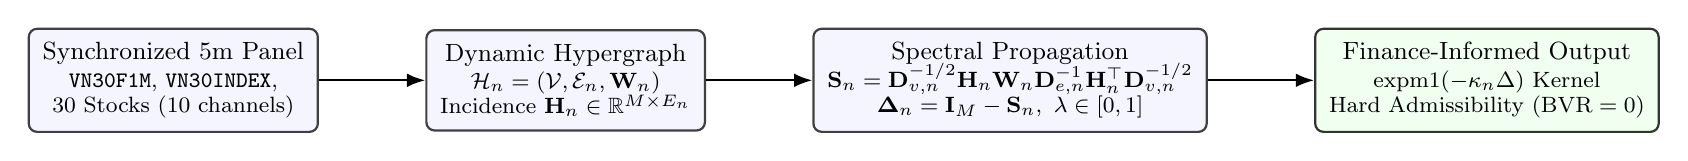
\begin{tikzpicture}[
    node distance=1.1cm and 1.35cm,
    >=Latex,
    box/.style={
        draw=black!75,
        rounded corners=3pt,
        thick,
        fill=blue!4,
        align=center,
        font=\small,
        minimum height=1.25cm,
        minimum width=2.85cm,
        inner sep=5pt
    },
    gatebox/.style={
        draw=black!80,
        rounded corners=3pt,
        thick,
        fill=green!6,
        align=center,
        font=\small,
        minimum height=1.25cm,
        minimum width=2.95cm,
        inner sep=5pt
    }
]
\node[box] (panel) {Synchronized 5m Panel\\[-1pt]\footnotesize\texttt{VN30F1M}, \texttt{VN30INDEX},\\[-2pt]\footnotesize 30 Stocks (10 channels)};
\node[box, right=of panel] (hgraph) {Dynamic Hypergraph\\[-1pt]\footnotesize $\mathcal{H}_n = (\mathcal{V}, \mathcal{E}_n, \mathbf{W}_n)$\\[-2pt]\footnotesize Incidence $\mathbf{H}_n \in \mathbb{R}^{M \times E_n}$};
\node[box, right=of hgraph] (lap) {Spectral Propagation\\[-1pt]\footnotesize $\mathbf{S}_n = \mathbf{D}_{v,n}^{-1/2}\mathbf{H}_n\mathbf{W}_n\mathbf{D}_{e,n}^{-1}\mathbf{H}_n^\top\mathbf{D}_{v,n}^{-1/2}$\\[-2pt]\footnotesize $\boldsymbol{\Delta}_n = \mathbf{I}_M - \mathbf{S}_n,\ \lambda \in [0, 1]$};
\node[gatebox, right=of lap] (adm) {Finance-Informed Output\\[-1pt]\footnotesize $\operatorname{expm1}(-\kappa_n \Delta)$ Kernel\\[-2pt]\footnotesize Hard Admissibility ($\text{BVR}=0$)};

\draw[->, thick] (panel) -- (hgraph);
\draw[->, thick] (hgraph) -- (lap);
\draw[->, thick] (lap) -- (adm);
\end{tikzpicture}
\end{document}
